% Options for packages loaded elsewhere
\PassOptionsToPackage{unicode}{hyperref}
\PassOptionsToPackage{hyphens}{url}
\PassOptionsToPackage{dvipsnames,svgnames,x11names}{xcolor}
%
\documentclass[
  letterpaper,
  DIV=11,
  numbers=noendperiod]{scrartcl}

\usepackage{amsmath,amssymb}
\usepackage{iftex}
\ifPDFTeX
  \usepackage[T1]{fontenc}
  \usepackage[utf8]{inputenc}
  \usepackage{textcomp} % provide euro and other symbols
\else % if luatex or xetex
  \usepackage{unicode-math}
  \defaultfontfeatures{Scale=MatchLowercase}
  \defaultfontfeatures[\rmfamily]{Ligatures=TeX,Scale=1}
\fi
\usepackage{lmodern}
\ifPDFTeX\else  
    % xetex/luatex font selection
\fi
% Use upquote if available, for straight quotes in verbatim environments
\IfFileExists{upquote.sty}{\usepackage{upquote}}{}
\IfFileExists{microtype.sty}{% use microtype if available
  \usepackage[]{microtype}
  \UseMicrotypeSet[protrusion]{basicmath} % disable protrusion for tt fonts
}{}
\makeatletter
\@ifundefined{KOMAClassName}{% if non-KOMA class
  \IfFileExists{parskip.sty}{%
    \usepackage{parskip}
  }{% else
    \setlength{\parindent}{0pt}
    \setlength{\parskip}{6pt plus 2pt minus 1pt}}
}{% if KOMA class
  \KOMAoptions{parskip=half}}
\makeatother
\usepackage{xcolor}
\setlength{\emergencystretch}{3em} % prevent overfull lines
\setcounter{secnumdepth}{-\maxdimen} % remove section numbering
% Make \paragraph and \subparagraph free-standing
\ifx\paragraph\undefined\else
  \let\oldparagraph\paragraph
  \renewcommand{\paragraph}[1]{\oldparagraph{#1}\mbox{}}
\fi
\ifx\subparagraph\undefined\else
  \let\oldsubparagraph\subparagraph
  \renewcommand{\subparagraph}[1]{\oldsubparagraph{#1}\mbox{}}
\fi


\providecommand{\tightlist}{%
  \setlength{\itemsep}{0pt}\setlength{\parskip}{0pt}}\usepackage{longtable,booktabs,array}
\usepackage{calc} % for calculating minipage widths
% Correct order of tables after \paragraph or \subparagraph
\usepackage{etoolbox}
\makeatletter
\patchcmd\longtable{\par}{\if@noskipsec\mbox{}\fi\par}{}{}
\makeatother
% Allow footnotes in longtable head/foot
\IfFileExists{footnotehyper.sty}{\usepackage{footnotehyper}}{\usepackage{footnote}}
\makesavenoteenv{longtable}
\usepackage{graphicx}
\makeatletter
\def\maxwidth{\ifdim\Gin@nat@width>\linewidth\linewidth\else\Gin@nat@width\fi}
\def\maxheight{\ifdim\Gin@nat@height>\textheight\textheight\else\Gin@nat@height\fi}
\makeatother
% Scale images if necessary, so that they will not overflow the page
% margins by default, and it is still possible to overwrite the defaults
% using explicit options in \includegraphics[width, height, ...]{}
\setkeys{Gin}{width=\maxwidth,height=\maxheight,keepaspectratio}
% Set default figure placement to htbp
\makeatletter
\def\fps@figure{htbp}
\makeatother
% definitions for citeproc citations
\NewDocumentCommand\citeproctext{}{}
\NewDocumentCommand\citeproc{mm}{%
  \begingroup\def\citeproctext{#2}\cite{#1}\endgroup}
\makeatletter
 % allow citations to break across lines
 \let\@cite@ofmt\@firstofone
 % avoid brackets around text for \cite:
 \def\@biblabel#1{}
 \def\@cite#1#2{{#1\if@tempswa , #2\fi}}
\makeatother
\newlength{\cslhangindent}
\setlength{\cslhangindent}{1.5em}
\newlength{\csllabelwidth}
\setlength{\csllabelwidth}{3em}
\newenvironment{CSLReferences}[2] % #1 hanging-indent, #2 entry-spacing
 {\begin{list}{}{%
  \setlength{\itemindent}{0pt}
  \setlength{\leftmargin}{0pt}
  \setlength{\parsep}{0pt}
  % turn on hanging indent if param 1 is 1
  \ifodd #1
   \setlength{\leftmargin}{\cslhangindent}
   \setlength{\itemindent}{-1\cslhangindent}
  \fi
  % set entry spacing
  \setlength{\itemsep}{#2\baselineskip}}}
 {\end{list}}
\usepackage{calc}
\newcommand{\CSLBlock}[1]{\hfill\break\parbox[t]{\linewidth}{\strut\ignorespaces#1\strut}}
\newcommand{\CSLLeftMargin}[1]{\parbox[t]{\csllabelwidth}{\strut#1\strut}}
\newcommand{\CSLRightInline}[1]{\parbox[t]{\linewidth - \csllabelwidth}{\strut#1\strut}}
\newcommand{\CSLIndent}[1]{\hspace{\cslhangindent}#1}

\KOMAoption{captions}{tableheading}
\makeatletter
\@ifpackageloaded{caption}{}{\usepackage{caption}}
\AtBeginDocument{%
\ifdefined\contentsname
  \renewcommand*\contentsname{Table of contents}
\else
  \newcommand\contentsname{Table of contents}
\fi
\ifdefined\listfigurename
  \renewcommand*\listfigurename{List of Figures}
\else
  \newcommand\listfigurename{List of Figures}
\fi
\ifdefined\listtablename
  \renewcommand*\listtablename{List of Tables}
\else
  \newcommand\listtablename{List of Tables}
\fi
\ifdefined\figurename
  \renewcommand*\figurename{Figure}
\else
  \newcommand\figurename{Figure}
\fi
\ifdefined\tablename
  \renewcommand*\tablename{Table}
\else
  \newcommand\tablename{Table}
\fi
}
\@ifpackageloaded{float}{}{\usepackage{float}}
\floatstyle{ruled}
\@ifundefined{c@chapter}{\newfloat{codelisting}{h}{lop}}{\newfloat{codelisting}{h}{lop}[chapter]}
\floatname{codelisting}{Listing}
\newcommand*\listoflistings{\listof{codelisting}{List of Listings}}
\makeatother
\makeatletter
\makeatother
\makeatletter
\@ifpackageloaded{caption}{}{\usepackage{caption}}
\@ifpackageloaded{subcaption}{}{\usepackage{subcaption}}
\makeatother
\makeatletter
\@ifpackageloaded{algorithm}{}{\usepackage{algorithm}}
\makeatother
\makeatletter
\@ifpackageloaded{algpseudocode}{}{\usepackage{algpseudocode}}
\makeatother
\makeatletter
\@ifpackageloaded{caption}{}{\usepackage{caption}}
\makeatother
\ifLuaTeX
  \usepackage{selnolig}  % disable illegal ligatures
\fi
\usepackage{bookmark}

\IfFileExists{xurl.sty}{\usepackage{xurl}}{} % add URL line breaks if available
\urlstyle{same} % disable monospaced font for URLs
\hypersetup{
  pdftitle={The Art of Scientific computation},
  colorlinks=true,
  linkcolor={blue},
  filecolor={Maroon},
  citecolor={Blue},
  urlcolor={Blue},
  pdfcreator={LaTeX via pandoc}}

\title{The Art of Scientific computation}
\usepackage{etoolbox}
\makeatletter
\providecommand{\subtitle}[1]{% add subtitle to \maketitle
  \apptocmd{\@title}{\par {\large #1 \par}}{}{}
}
\makeatother
\subtitle{A survey of techniques for simulation of the abelian sandpile
model}
\author{James Reuben Bender}
\date{2024-10-26}

\begin{document}
\maketitle

\floatname{algorithm}{Algorithm}

\section{Introduction}\label{introduction}

\subsection{The abelian sandpile
model}\label{the-abelian-sandpile-model}

The abelian sandpile model is a cellular automaton inspired by the
casding behaviour of collections of sand grains piled to a critical
height Bak, Tang, and Wiesenfeld (1988) . Often, and hereafter, referred
to as the Bak-Tang-Weisenfeld (BTW) model after its early investigators
Bak, Tang, and Wiesenfeld (1987), the model has become a prototypical
example of `self-organised criticality' in physical systems Dhar (1990)
and has inspired numerous extensions (see Járai (2018) for review).

The BTW model is defined on a lattice, where each point (`site') holds
some number of sand grains (i.e.~can be thought of as being at certain
`height'). When a particular number of grains accumulate on a site, the
pile becomes unstable and \emph{topples} sending grains to its neighbors
(itsef losing that number of grains). This spread of sand grains can
cause a chain reaction of topplings -an `avalanche'- that can propagate
through the lattice. While each topple is simple and deterministic,
predicting the size and shape of the avalanches on a large lattice with
an arbitrary height distribution can be non-trivial - a problem
compounded as we model the behaviour of the system over time (i.e.~as we
sequentially add grains). Therefore, the abelian sandpile model is a
good candidate for computational simulation. By repeating the
toppling/avalanche process iteratively, we may characterize features of
the sandpile model (e.g.~the distribution of avalanche sizes, the
average number of grains present on the lattice, or any apparent
equilibrium states) statistically rather than analytically.

This project aims to present methods of simulating the BTW model.

When using a finite grid and losing grains at the edges, our output is
subject to so called `finite size effects', whereby extreme events are
less common than we would expect on an infinite grid. This is because
the avalanches are more likely to be cut off by the boundaries. To a
\#\#\# Applications of the BTW model e.g.~simulation of physical
systems, traffic flow, forest fires, epidemiological models etc. \#\#
Scientific programming tools

In large sandpiles, which have the potential for large scale avalanves
(e.g.~involving millions of topples), the computational tools and
techniques used to simulate the model are crucial. A secomdary aim of
this progject (in adittion to presenting the BTW model) is to explore
several alternative computational techniques for developing and
simulating the model. There are two main aspects I will consider:

Algorithm design: The way in which the toppling and stabilisation
algorithms implemented can have a significant impact on the efficiency
of the simulation. These design decisions will depend on the backend on
which the simulation is run - e.g.~Does the algorithm complexity scale
efficiently with the lattice size (to avoid memory bottlenecks)? Can the
algorithm make use of the multithreading capabilities of modern CPUs
(or, moreover, GPUs)? Therefore, there is unlikely to be a single
optimal algorithm, but rather a trade-off between different factors. I
will compare the performance of several different algorithms for
simulating the BTW model.

Programming languages: The choice of programming language can also have
a significant impact on the efficiency of simulation; both in the sense
of the time taken to run the simulation, and the ease of developing and
maintaining code. Modern scientific programming typically falls into a
two-language paridigm, wherein a relatively high-level, dynamic language
(usually python) is used for rapid prototyping and data analysis, and a
lower-level, statically typed and compiled language (e.g.~C, C++,
Fortran) is used for computationally intensive tasks. There is some
middle ground here with the use of high level wrappers in dynamic
languages that call high performance compiled code for performance
critical tasks (e.g.~numpy, scipy, numba in python).

While these approaches well established and can result in highly
efficient implimentations, the two language approach has drawbacks. The
most obvious is the need to develop (and potentially maintain) two
separate codebases. Moreover, the specialised skills needed to develop
and maintain high performance code in a low-level language can be a
barrier to entry for many researchers. This barrier can be compounded by
the discontinuity in source material between two codebases. For example,
localising and adressing bugs can require more elaborate error handling
and logging when the code is split between two languages.

The Julia language was developed as an alternative to the two-language
approach @. A high level, dynamic language Julia's progressive typing
and type inference system, along with just-in-time compilation, intends
to allow for easily readable and maintainable code that can be optimised
for performance without leaving the language - a language that `walks
like python, runs like C'.

This report will present a comparison of the performance of several
different algorithms for simulating the BTW model, implemented in Julia
and python. The aim is to explore the trade-offs between algorithm
design and programming language choice, and to potentially to inform
students or researchers devevloping their own simulations of the BTW
model.

\section{Part 1: Implimenting a naive model is several programming
languages}\label{part-1-implimenting-a-naive-model-is-several-programming-languages}

\subsection{Basic toppling and stabilisation
algorithms}\label{basic-toppling-and-stabilisation-algorithms}

\subsubsection{the `push' topple
algorithm}\label{the-push-topple-algorithm}

The push algorithm is a simple way to implement the toppling of a site
in a sandpile model. The implimentation follow the intuitive desription
of the toppling process: if a certain site \(X_ij\) is at/above the
height threshold \(k\), and so is unstable. stabilisiation of this site
occurrs by distributing its grains to it's four neighbours. i.e.~each of
\({X_{i-1,j}, X_{i+1,j}, X_{i,j-1}, X_{i,j+1}}\) recieves one grain and
\(X_ij\) looses four grains. Figure~\ref{fig-pushtopple}

\begin{figure}

\centering{

\captionsetup{labelsep=none}
\includegraphics{index_files/mediabag/figures/push_topple.pdf}

}

\caption{\label{fig-pushtopple}}

\end{figure}%

\begin{algorithm}[htb!]
\caption{Push toppling algorithm}
\label{alg-pushtopple}
\begin{algorithmic}[1]
  \If {$X_{i} \geq k$}
      \State $Y_{i} \gets X_{i} - k$
      \For{each neighbor $j$ of $i$}
          \State $Y_j \gets X_j + 1$
      \EndFor
  \Else
      \State $Y_i \gets X_i$
  \EndIf 
\end{algorithmic}
\end{algorithm}

\subsubsection{Naive stabilisation
algorithm}\label{naive-stabilisation-algorithm}

The naive stabilisation algorithm is naive in in the sense that it does
not assume any information about where topples might occur (i.e.~it
checks every site, c.f.the targeted algorithm). The algorithm iterates
over each site in the lattice applying a toppling rule (e.g.~the push
algorithm) until no sites are above the threshold.

\begin{algorithm}[htb!]
\caption{Naive stabilisation algorithm}
\label{alg-naivestabilise}
\begin{algorithmic}[1]
\While {any site in $X$ is above $k$}
  \For {each site $i$ in $X$}
      \If {$X_i \geq k$}
          \State $Y$ $\gets$ topple!(X, i)
      \Else
          \State $Y_i$ $\gets$ $X_i$
      \EndIf 
  \EndFor
\EndWhile
\end{algorithmic}
\end{algorithm}

\subsection{Benchmarking setup}\label{benchmarking-setup}

To compare the performance across languages, a consistent test setup is
needed. Thankfully, the deterministic nature of the sandpile model
allows the simple construction of sandpiles with known stabilisation
times. Given a NxN lattice, test sandpiles can be constructed by filling
the central \(3 < n< N\) sites of an empty lattice with \(k-1\) grains.
addition of a single grain at the center of the lattice will cause
increasing number of topplings as \(n\) increases. Such regular grids
will be used to test the performance of implementations of the naive
push stabilisation algorithm in python, and julia. Specific
implimentations of the algorithm in each language are given in appendix
1.

\subsection{Results}\label{results}

The performance of the naive stabilisation algorithm was tested on a
101x101 lattice with \(k=4\) grains. The number of topplings required to
stabilise the lattice was recorded for each \(n\) in the range
\(3 < n < 100\). The results are shown in Figure~\ref{fig-languageperf}

\begin{figure}

\centering{

\captionsetup{labelsep=none}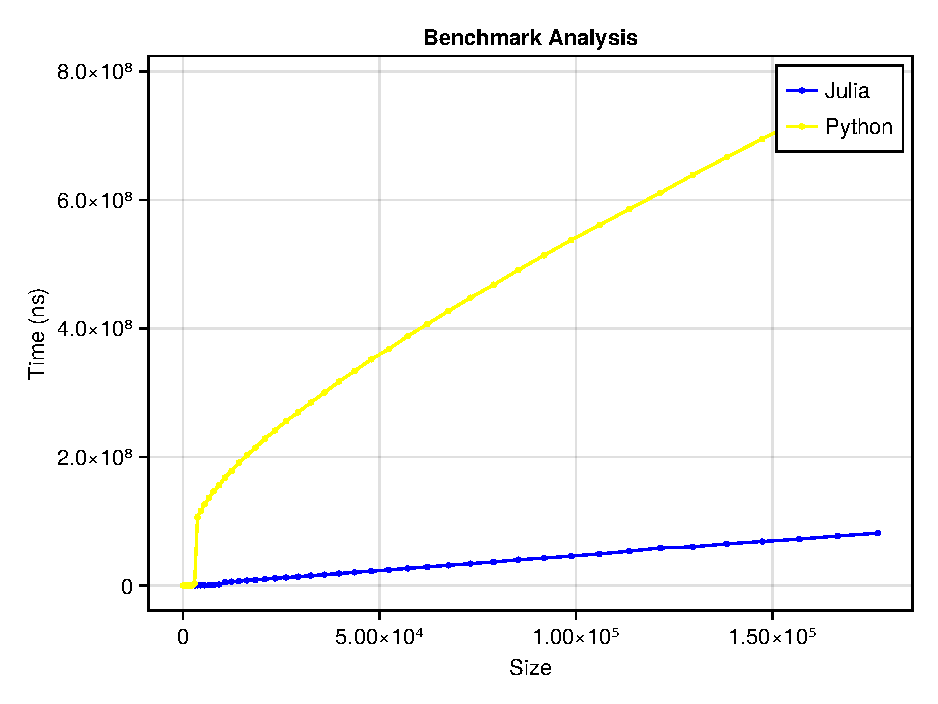
\includegraphics{figures/language_stabilisation_benchmark.pdf}

}

\caption{\label{fig-languageperf}}

\end{figure}%

\phantomsection\label{refs}
\begin{CSLReferences}{1}{0}
\bibitem[\citeproctext]{ref-bak_self-organized_1987}
Bak, Per, Chao Tang, and Kurt Wiesenfeld. 1987. {``Self-Organized
Criticality: An Explanation of the 1/f Noise.''} \emph{Physical Review
Letters} 59 (4): 381--84.
\url{https://doi.org/10.1103/PhysRevLett.59.381}.

\bibitem[\citeproctext]{ref-bak_self-organized_1988}
---------. 1988. {``Self-Organized Criticality.''} \emph{Physical Review
A} 38 (1): 364--74. \url{https://doi.org/10.1103/PhysRevA.38.364}.

\bibitem[\citeproctext]{ref-dhar_self-organized_1990}
Dhar, Deepak. 1990. {``Self-Organized Critical State of Sandpile
Automaton Models.''} \emph{Physical Review Letters} 64 (14): 1613--16.
\url{https://doi.org/10.1103/PhysRevLett.64.1613}.

\bibitem[\citeproctext]{ref-jarai_sandpile_2018}
Járai, Antal A. 2018. {``Sandpile Models.''} \emph{Probability Surveys}
15 (January). \url{https://doi.org/10.1214/14-PS228}.

\end{CSLReferences}



\end{document}
